\section{Amplifying local endpoint maps}\label{amp:section}

Throughout this section percolation has parameter $\pc$, and the automorphism
group is unimodular.  We use the weighted transport identity
\eqref{eq:s02}, the walk bound \eqref{eq:s03}, critical finiteness, and the
goodness estimate \eqref{eq:s06}.  The purpose of the construction is to turn
a heavy cluster-size tail into a local rule whose endpoint spreads very
widely relative to its probability of success and its cluster-size cap.
The next section will show that such rules contradict the heavy tail.

Suppose that
\begin{equation}\label{eq:s09}
 [\E_{\pc}s_o^\alpha]=\infty
 \qquad\text{for some }0<\alpha<\tfrac12.
\end{equation}
Choose $\beta>\alpha$ and $\epsilon>0$ so that, with
$s=\tfrac12+\epsilon$, we have $\beta+s<1$.  Goodness below always uses this
choice of $s$.

\subsection{One orbit and a sequence of scales}\label{amp:scales-section}

\begin{lemma}[Selection of an orbit]\label{amp:scales}
There are a vertex orbit $O$, a constant $c>0$, and an unbounded sequence
$\mathcal N$ of dyadic integers such that, for $n\in\mathcal N$ and
$\pi=[\Prob_{\pc}(n\le s_o<2n)]$,
\begin{equation}\label{eq:s10}
 \begin{split}
 \pi&\ge n^{-\beta},\\
 [\Prob_{\pc}(n/2\le s_o<2n)]&\le(1+2^\beta)\pi,\\
 \E_{\pc}\bigl[|C_x\cap O|\one_{\{n\le s_x<2n\}}\bigr]
     &\ge c n\pi\qquad(x\in O).
 \end{split}
\end{equation}
The orbit and the sequence can be kept fixed throughout the amplification.
\end{lemma}

\begin{proof}
Put $\pi_j=[\Prob_{\pc}(2^j\le s_o<2^{j+1})]$.  The sequence
$2^{\beta j}\pi_j$ is unbounded: a uniform bound would make
$\sum_j2^{\alpha j}\pi_j$ finite, contrary to \eqref{eq:s09}.
Choose its successive record indices, omitting an initial finite segment
so that their record values are at least one.  At a record index $j$,
$\pi_{j-1}\le2^\beta\pi_j$, proving the first two assertions.

Let $h$ be the number of vertex orbits.  Call a vertex of a finite cluster
qualifying if its orbit occupies at least $1/h$ of the cluster.  At least
$1/h$ of the vertices of every cluster qualify.  Transport, uniformly
within each finite cluster in the chosen bin, gives
\[
 [\Prob_{\pc}(n\le s_o<2n,\ o\text{ qualifies})]
 =\left[\E_{\pc}\left[
   \one_{\{n\le s_o<2n\}}
   \frac{\#\{v\in C_o:v\text{ qualifies}\}}{s_o}\right]\right]
 \ge\frac\pi h.
\]
For at least one type $i$, its contribution to the left side is at least
$\pi/h^2$.  At a representative $x$ of this type,
\[
 \E_{\pc}\bigl[|C_x\cap O_i|\one_{\{n\le s_x<2n\}}\bigr]
 \ge \frac n h\,
      \Prob_{\pc}(n\le s_x<2n,\ x\text{ qualifies})
 \ge \frac{n\pi}{h^3\sigma_i}.
\]
One of the finitely many types is selected along an unbounded subsequence
of record scales.  Keep that subsequence and write $O$ for its orbit.
\end{proof}

\begin{definition}[Local endpoint map]\label{amp:map}
A local endpoint map on $O$ is a randomized rule at each $x\in O$ that
reads percolation bits in a deterministic finite ball about $x$ and uses
auxiliary randomness independent of those bits.  Its conditional rules
are covariant under automorphisms.  The rule either fails or outputs
$y\in C_x\cap O$.  A map with integer cap $M$ is required, on every successful
input pattern, to have $s_x\le M$ and $C_x$ good for cap $M$.

Write $u>0$ for its success probability and
\[
 \begin{gathered}
 K(x,y)=\Prob(\text{output }y\mid\text{success at }x),
 \qquad r=\norm K,\\
 U=\log(1/u),\quad m=\log M,\quad H=\log(1/r).
 \end{gathered}
\]
All probabilities here include the auxiliary randomness, and the operator
norm is on counting-measure $\ell^2(O)$.
\end{definition}

Invariance makes $u$ independent of $x\in O$.  The kernel $K$ has row sums
one; transport restricted to $O\times O$ gives column sums one as well.
Thus $0<r\le1$ by the row and column sum bound.  Symmetry of $K$ is neither
assumed nor needed.

\begin{proposition}[Efficient endpoint maps]\label{amp:efficient-maps}
Under \eqref{eq:s09}, for every $\eta>0$ there is a local endpoint map on
the orbit $O$ of \cref{amp:scales}, with $M\ge2$ and $H>1$, such that
\[
 \frac{U+m}{H}<\eta.
\]
Moreover the maps can be chosen so that $H$ tends to infinity.  Their
radii are finite, but need not be bounded uniformly over the construction.
\end{proposition}

We prove the proposition by constructing a starting map, establishing
one amplification step, and then specifying the order of all parameters.

\begin{lemma}[Starting map]\label{amp:initial}
There is a local endpoint map on $O$ with $H>1$, with cap as large as
prescribed.
\end{lemma}

\begin{proof}
From $x\in O$ sample a length-$\ell$ walk with kernel $P$, independently of
percolation.  Require its endpoint to lie in $O$ and all distinct edges
traversed by the walk to be open.  If $e$ is the number of distinct
traversed edges, accept also an independent coin of probability
$\pc^{\ell-e}$.  Holding steps do not count as edges.  Before imposing a
cluster cap, the resulting endpoint mass kernel is exactly
$\pc^\ell P^\ell|_{O\times O}$.  The finite type chain gives, for all large
$\ell$, a row sum at least $c_1\pc^\ell$, with $c_1>0$ independent of
$\ell$.  Its norm is at most $\pc^\ell\rho^\ell$.

Fix $\ell$ large enough that $2\rho^\ell/c_1<e^{-1}$.  Critical finiteness
and \eqref{eq:s06} allow us to choose any sufficiently large $M$ and reject
unless $s_x\le M$ and $C_x$ is good for cap $M$, losing at most half the
preceding lower bound on the row sum.  Entrywise domination by the uncut
mass kernel gives $r\le2\rho^\ell/c_1<e^{-1}$.  The capped cluster and its
goodness can be tested in a deterministic finite ball, so this is a local
map.
\end{proof}

\subsection{Splicing independent clusters}\label{amp:splicing-section}

Fix an old map with parameters $(u,M,r)$, an integer $k\ge1$, and a scale
$n\in\mathcal N$ such that $kM\le n/2$.  Constants in what follows may
depend on the graph and the fixed choices $\beta,\epsilon,O$, but not on
$n,k$ or the old map unless stated otherwise.

All finite choices can be made covariantly using independent continuous
priorities on vertices or edges.  More explicitly, keep three independent
families of seeds: the old-map seeds, priorities ordering new contact
lists, and a uniform random variable $V_i\in[0,1]$ for the contact choice
at each possible index $1\le i\le k$.  Ties in priorities have probability
zero and may be rejected.  An automorphism permutes the seed indices and
preserves their joint law, so this realization does not require a free
action or a choice of an automorphism carrying one root to another.
A rule with already integrated endpoint probabilities is likewise
realized by a categorical draw using its old-map seed.  Once those seeds
are fixed, old rules can be replayed deterministically.

For fixed $x,z\in O$ perform the following experiment.  In a distinguished
independent field $D$, require
$A=C_x(D)$ to satisfy $n\le|A|<2n$.  Independently, start at $z$ and take
$k$ old-map steps, using a new independent percolation field and new seeds
for each step.  Give the experiment mass $1/n$ if every step succeeds and
the last endpoint lies in $A$, and zero otherwise.  A successful chain,
listed in reverse order, has vertices
\[
 y_0\in A,\quad y_1,\ldots,y_k=z.
\]
Let $E_i$ be the field used between $y_i$ and $y_{i-1}$, and let $C_i$ be
its whole open cluster containing these vertices.  Each $C_i$ is good for
cap $M$ and has at most $M$ vertices.  This reversal is only a way of
listing a realized chain; it makes no reversibility assertion about $K$.

Starting with $S=A$, apply the following switching procedure until
$z\in S$.  Select the largest still eligible index $i$ for which
$C_i\cap S\ne\varnothing$; after this selection only indices larger than
$i$ remain eligible.  Let $B_i$ be the component of $y_i$ in the open
subgraph of $E_i$ induced by $V\setminus S$.  Among its $K_i$ open
$E_i$-edges to $S$, choose one edge $e_i$ uniformly.  Exchange the $D$ and
$E_i$ bits on the mask
\[
 \{e_i\}\ \cup {}
 \{e:e\text{ is incident to }B_i
             \text{ and both endpoints of }e\text{ lie outside }S\}.
\]
The field $D$ in this instruction is its current value.

\begin{lemma}[Geometry of the switching procedure]\label{amp:splicing}
Every step is well defined.  Its effect on the distinguished root cluster
is exactly $S\mapsto S\cup B_i$.  The selected indices increase, and the
inserted pieces form a chain, each attached to the preceding piece by
one open bridge $e_i$; the first piece is attached to $A$.
Every selected bridge separates $x$ from $z$ in the final distinguished
field $D'$, and
\begin{equation}\label{eq:s11}
 z\in C_x(D'),\qquad s_x(D')\le M'=2n+kM.
\end{equation}
\end{lemma}

\begin{proof}
Initially an eligible intersecting cluster exists because $y_0\in A$.
After a selection at $i$, the new set contains $y_i$, so if $i<k$ and
$z$ has not been reached, $C_{i+1}$ supplies another eligible intersection.
The selected $y_i$ lies outside the current $S$: if $i<k$ and $y_i\in S$,
then $C_{i+1}$ would intersect $S$, contradicting maximality; if $i=k$,
this would contradict the stopping condition.  Since $C_i$ is connected
and meets $S$, the component $B_i$ has $K_i\ge1$ open contacts with $S$.

Before the exchange, all $D$-edges leaving $S$ are closed.  The exchange
imports the internal open connections of $B_i$ and its closed boundary
to $V\setminus(S\cup B_i)$ from $E_i$, and opens the chosen contact
$e_i$.  Every other contact to $S$ keeps its closed $D$ bit.  No edge
internal to $S$ changes.  Hence the new root cluster is exactly
$S\cup B_i$, with $e_i$ its sole open contact between the two parts.

Every index larger than the selected $i$ missed the entire pre-switch
$S$.  Consequently the next selected cluster can contact the enlarged
root cluster only through $B_i$.  Applying this observation at each step
shows that later pieces attach to their immediate predecessors and do
not acquire open contacts with earlier pieces.  Thus all the seams
remain bridges, and, when the procedure stops, separate $x$ from
$z$ in their natural order.  There are at most $k$ inserted pieces,
each of size at most $M$, proving \eqref{eq:s11}.
\end{proof}

\Cref{fig:splicing} illustrates the chain of inserted pieces.  The
separating seams will let us recover the original fields from the
switched fields once the seam locations have been recorded.
\begin{figure}[tbp]
\centering
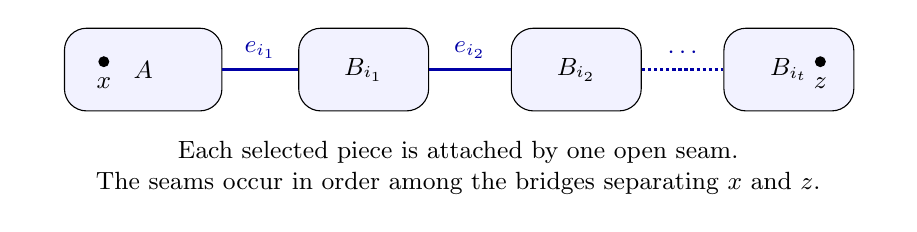
\begin{tikzpicture}[x=1cm,y=1cm,font=\small,
  piece/.style={draw,rounded corners=8pt,fill=blue!5,minimum width=1.65cm,minimum height=1.05cm},
  seam/.style={very thick,blue!65!black},dot/.style={circle,fill,inner sep=1.4pt}]
\node[piece,minimum width=2cm] (a) at (0.3,0) {$A$};
\node[piece] (b1) at (3.1,0) {$B_{i_1}$};
\node[piece] (b2) at (5.8,0) {$B_{i_2}$};
\node[piece] (bt) at (8.5,0) {$B_{i_t}$};
\draw[seam] (a.east)--node[above] {$e_{i_1}$} (b1.west);
\draw[seam] (b1.east)--node[above] {$e_{i_2}$} (b2.west);
\draw[seam,densely dotted] (b2.east)--node[above] {$\cdots$} (bt.west);
\node[dot,label=below:$x$] at (-0.2,0.10) {};
\node[dot,label=below:$z$] at (8.9,0.10) {};
\node[align=center,text width=10.7cm] at (4.3,-1.25)
{Each selected piece is attached by one open seam.\\
The seams occur in order among the bridges separating $x$ and $z$.};
\end{tikzpicture}
\caption{The chain produced by the switching procedure. Cutting the
selected seams recovers the inserted pieces and the initial cluster
$A$. The drawing shows vertex sets and selected open seams, with
internal edges and other incident edges omitted.}
\label{fig:splicing}
\end{figure}


\subsection{Coding an inverse and defining its load}\label{amp:coding-section}

\begin{lemma}[Inverse codes and contact probabilities]\label{amp:coding}
Fix the output fields, $x,z$, the old-map seeds, and the priorities
ordering contact lists.  A valid switching input can be specified by the
selected indices and positive gaps locating the selected seams in the
ordered list of bridges separating $z$ from $x$, read from $z$ toward
$x$.  Each fixed code determines at most one input bit tuple, without
using the fresh contact uniforms.  After integrating those uniforms, the
total mass of valid codes is at most
\begin{equation}\label{eq:s12}
 W^k,\qquad
 W=1+\sum_{l=1}^{M}\min\{1,2M^s/l\}
       \le C M^s\log M.
\end{equation}
\end{lemma}

\begin{proof}
List the selected indices in decreasing order, hence their seams in the
order encountered from $z$ toward $x$.  The code records the number of
separating bridges up to each next seam, counting that seam.  Cutting
the indicated seams in the final root cluster recovers the inserted
pieces and $A$, since \cref{amp:splicing} gives exactly a chain of singly
attached connected pieces.  Thus it determines every pre-switch set
$S$, every $B_i$, and every exchange mask.  Undo these masks in reverse
chronological order.  The candidate input tuple is now fixed, and the
old rules can be replayed from $z$ to check all their successes, their
endpoints, and the prescribed selection rule.  An invalid code is simply
discarded.

Let $l_i$ be the gap ending at seam $e_i$.  Other than that seam, its
bridges lie inside $B_i$, between the attachment point toward $z$ and
the attachment point toward $x$.  Therefore $l_i\le|B_i|\le M$.
Deleting the pre-switch set $S$ from the original good cluster $C_i$
leaves $B_i$ with $K_i$ original open contacts.  Goodness bounds its
pivotal diameter by $K_iM^s$.  Since no later piece supplies a bypass,
\[
 l_i\le1+K_iM^s,
 \qquad
 \frac1{K_i}\le\min\{1,2M^s/l_i\}.
\]
For the second inequality use $K_i\ge1$ if $l_i=1$, and
$l_i-1\ge l_i/2$ otherwise.

The reconstruction just given has not consulted any $V_i$.  In the
reconstructed input, each contact list and its priority order are fixed.
If its prescribed seam has rank $a_i$ among $K_i$ contacts, the fresh
uniform must lie in
$[(a_i-1)/K_i,a_i/K_i)$.  These intervals are determined without any of
the fresh uniforms, so their product Lebesgue measure is
$\prod_iK_i^{-1}$.  Any further validity restrictions only decrease it.
The priorities are integrated once under their probability law, rather
than counted as additional inverse choices.  Summing over a skipped
index or a gap $1\le l\le M$ at each index proves the bound $W^k$.
Finally the harmonic sum gives $W\le C M^s\log M$ for $M\ge2$.
\end{proof}

For clarity, all measure comparisons here can be made on finite bit
spaces.  In a successful experiment the chain connects $z$ by at most
$kM$ edges to a vertex of the connected set $A$, so
$\dist(x,z)\le2n+kM$.  A capped whole-cluster test exposes the boundary
or stops as soon as the cap is exceeded.  The old rule has a fixed query
radius, and its successful steps move at most $M$.  Consequently a
deterministic larger ball about $x$ contains every query and every
exchange mask for every successful experiment.  There are finitely many
candidate endpoints and codes.  When checking an inverse, stop at the
first failed capped test or failed old step; this uses a deterministic
larger ball as well.  Conditioning on all bits outside this ball reduces
every comparison to finitely many Bernoulli coordinates.

At fixed seeds, the exchanges preserve the total number of open bits
among equally distributed fields.  Thus each input bit tuple and its
output have exactly the same product probability, even though the
exchange masks depend on the input.  The injective inverse with a fixed
code therefore gives the following exact density description.  For a
single reference iid distinguished field $D'$, let
$L_x(z,D')$ be $1/n$ times the sum of valid inverse-code indicators,
integrated over reference iid auxiliary output fields and all independent
seeds.  The preceding finite comparison says that this is the density
of the switched mass at $z$ relative to the law of $D'$.  In particular,
\[
 0\le L_x(z,D')\le W^k/n.
\]
After the auxiliary integrations these are covariant local functions
of $D'$, supported on \eqref{eq:s11}.  Put
$L=\sum_{z\in O}L_x(z,D')$ and $b_0=\E L$.
The reference product law in this definition is not a claim that the
actual output of a switch has independent fields, or that its contact
coins remain independent after conditioning on that output.

\begin{lemma}[Mean load]\label{amp:mean}
With $F(x,z)=\E L_x(z,D')$, one has
\begin{equation}\label{eq:s13}
 \begin{split}
 F(x,z)&=\frac{u^k}{n}\sum_{y\in O}
  \Prob_{\pc}(y\in C_x,\ n\le s_x<2n)K^k(z,y),\\
 c\pi u^k&\le b_0\le C\pi u^k,
 \qquad \norm{F/b_0}\le r^k.
 \end{split}
\end{equation}
\end{lemma}

\begin{proof}
The density comparison preserves total mass, so the mean is computed
in the original experiment.  The $k$ independent old steps have
unconditional endpoint kernel $u^kK^k$, giving the displayed formula.
Let
\[
 B_n(x,y)=\Prob_{\pc}(y\in C_x,\ n\le s_x<2n),\qquad x,y\in O.
\]
This is symmetric: on $y\in C_x$, the two root clusters coincide.
Its row sum $b_n$ is constant on $O$, and by \eqref{eq:s10} and
$\Prob_{\pc}(n\le s_x<2n)\le\pi/\sigma_O$,
\[
 cn\pi\le b_n\le2n\pi/\sigma_O.
\]
Here $\sigma_O$ is the type weight of $O$.  Since $K^k$ has column sums
one, $b_0=u^kb_n/n$.  Moreover
$F/b_0=(B_n/b_n)(K^k)^*$, where $*$ denotes transpose.  The symmetric
stochastic kernel $B_n/b_n$ has norm at most one, proving the norm bound.
\end{proof}

\subsection{The second moment}\label{amp:second-moment-section}

The mean kernel already has norm at most $r^k$ after normalization.
To turn $L_x(z,D')$ into output probabilities, however, we must control
the fields on which its total load $L$ is large.  The next estimate will
let us truncate those fields while retaining a fixed fraction of the
mean.  The distinction between an underlying graph edge and an open
edge is essential in its proof.

\begin{lemma}[Second moment of the load]\label{amp:second-moment}
There is a fixed polynomial $Q(k,M)\ge1$ such that
\begin{equation}\label{eq:s14}
 \E L^2\le Q(k,M)\pi u^{2k}
 \qquad\text{whenever } kM\le n/2
               \text{ and } n\ge(W/u)^k.
\end{equation}
\end{lemma}

\begin{proof}
Write $v=kM$.  Expand $L^2$ using a common reference distinguished field
$D'$ and two independent families of auxiliary output fields and seeds.
Thus an individual summand consists of two valid coded inverses with
endpoints $z_1,z_2$.  We divide the summands into three classes.

\paragraph{At least one inverse makes no switch.}
Let $L_0$ be the integrated part of $L$ with no switch.  In this case
$A=C_x(D')$ is in the bin and $z\in A$.  Ignoring any further conditions
and summing the old-chain mass gives
\[
 L_0\le\frac{u^k}{n}\one_{\{n\le|A|<2n\}}
          \sum_{z\in A\cap O}\sum_{y\in A\cap O}K^k(z,y)
 \le 2u^k,
\]
by the column sums.  Summands with at least one such factor contribute
at most $2\E[L_0L]\le4u^kb_0\le C\pi u^{2k}$.

\paragraph{The two hanging components are nested or adjacent.}
For a nonempty switching inverse, let $B$ be the component beyond its
first seam, viewed from $x$ in $C_x(D')$.  By \cref{amp:splicing}, $B$ is
exactly the union of the inserted pieces, contains its endpoint $z$,
and has at most $v$ vertices.  Two such hanging components in the same
rooted bridge tree are either nested or disjoint.

Fix the first inverse and its $B^1,z_1$.  There are at most
\[
 N_v=v+v^2+dv^3
\]
possible second endpoints among pairs for which the hanging components
are nested or joined by an underlying graph edge.  Indeed, if
$B^2\subseteq B^1$, there are at most $v$ endpoints.  If
$B^1\subseteq B^2$, the first seam of $B^2$ is one of the last $v$
separating bridges on the route from $x$ to $z_1$.  Each seam determines
one hanging component and supplies at most $v$ endpoints when that
component is small enough.  This gives $v^2$.  Finally, for disjoint
adjacent components, choose a vertex of $B^2$ neighboring $B^1$ in at
most $dv$ ways; its seam is among the last $v$ separating bridges on
the route to that vertex, and each resulting component contains at
most $v$ possible endpoints.  This gives $dv^3$.

For each endpoint, \cref{amp:coding} bounds the integrated second
inverse mass by $W^k/n$.  Integrating the first inverse therefore bounds
this class by
\[
 b_0N_v\frac{W^k}{n}\le C N_v\pi u^{2k},
\]
using $n\ge(W/u)^k$.

\paragraph{The hanging components are disjoint and graph-nonadjacent.}
Now suppose $B^1$ and $B^2$ are disjoint and no edge of the underlying
graph joins them.  Every distinguished-field edge exchanged by inverse
$a$ is incident to $B^a$.  Hence the two collections of masks are
disjoint, including their seams.  Undo both inverses.  In the jointly
restored distinguished field $D_{00}$ the exact root cluster is
\begin{equation}\label{amp:joint-root}
 A_{00}=C_x(D')\setminus(B^1\cup B^2),
 \qquad n-v\le|A_{00}|<2n.
\end{equation}
To verify the first assertion, removing two disjoint hanging components
leaves a connected set containing $x$.  Its contacts with each removed
component are closed by that inverse, and are untouched by the other
inverse.  Its other boundary edges remain closed.  For the size bound,
either single inverse starts from
$A^a=C_x(D')\setminus B^a$ of size in $[n,2n)$, and removing the other
component loses at most $v$ vertices.

The geometry of this joint restoration is shown in
\cref{fig:joint-inverse}.
\begin{figure}[tbp]
\centering
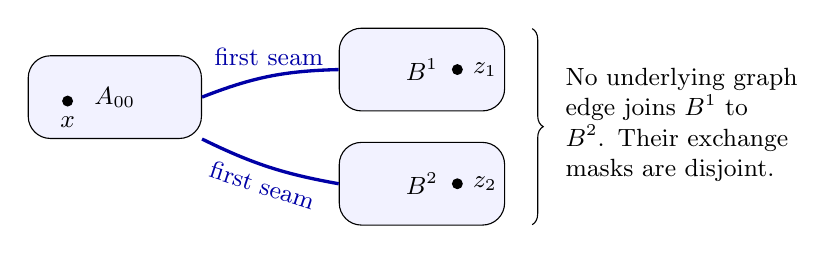
\begin{tikzpicture}[x=1cm,y=1cm,font=\small,
  piece/.style={draw,rounded corners=8pt,fill=blue!5,minimum width=1.65cm,minimum height=1.05cm},
  seam/.style={very thick,blue!65!black},dot/.style={circle,fill,inner sep=1.4pt}]
\node[piece,minimum width=2.2cm] (root) at (0.4,0) {$A_{00}$};
\node[piece,minimum width=2.1cm] (upper) at (4.3,.35) {$B^1$};
\node[piece,minimum width=2.1cm] (lower) at (4.3,-1.1) {$B^2$};
\draw[seam] (root.east) to[bend left=10] node[above] {first seam} (upper.west);
\draw[seam] (root.south east) to[bend right=8] node[below,sloped] {first seam} (lower.west);
\node[dot,label=below:$x$] at (-0.2,-.05) {};
\node[dot,label=right:$z_1$] at (4.75,.35) {};
\node[dot,label=right:$z_2$] at (4.75,-1.1) {};
\draw[decorate,decoration={brace,amplitude=4pt}] (5.7,.87)--(5.7,-1.62);
\node[align=left,anchor=west,text width=3cm] at (6,-.35)
{No underlying graph edge joins $B^1$ to $B^2$. Their exchange masks are disjoint.};
\end{tikzpicture}
\caption{Two hanging components in a common switched root cluster.
Undoing both insertions leaves $A_{00}$. Graph nonadjacency makes
the two collections of exchange masks disjoint. The proof recovers
each insertion from the jointly restored fields. The open seams
shown belong to the switched configuration; internal and other
incident edges are omitted.}
\label{fig:joint-inverse}
\end{figure}


We claim that, at fixed $z_1,z_2$ and all seeds, joint undoing is injective
without retaining either code.  This stronger assertion removes the
factor $W^{2k}$ from this class.  The restored auxiliary fields and
old-map seeds first recover both entire old chains by replay from their
endpoints; the distinguished field is irrelevant to that replay.
Run the first switching procedure virtually from $A_{00}$ with its
restored chain.  Here ignore only the original bin test and the test
that $y_0\in A$; keep the maximal-index selection and stopping rules.
We show inductively that its current set is $S_0=S\setminus B^2$, where
$S$ is the corresponding current set in the original first forward run,
and that the same index, component, contact and mask are selected.

Let $i$ be the original selected index and write its seam as
$e_i=(a_i,b_i)$ with $a_i\in S$ and $b_i\in B_i^1\subseteq B^1$.
Graph nonadjacency forces $a_i\notin B^2$, so the selected old cluster
still meets $S_0$.  Every larger eligible index missed $S$ and therefore
misses $S_0$.  Thus maximality chooses the same $i$.  This remains true
when unused trajectory clusters meet $B^2$, or even when the original
$y_0$ belongs to $B^2$.

Replacing $S$ by $S_0$ admits only the vertices of $B^2$ to the slit
domain.  If the component $B_i^1$ enlarged, an enlarging open path would
have a first vertex in $B^2$.  The preceding part of that path lies in
the old slit domain, hence in $B_i^1$.  Its next edge would join $B^1$
to $B^2$, a contradiction.  Thus the slit component is unchanged.
Its contact list and its exchange mask are also unchanged, since their
only possible differences would be edges between $B_i^1$ and $B^2$.
The fixed priorities and contact uniform choose the same seam.  The
other undoing changed no bit on this mask.  After the exchange the
inductive relation $S_0=S\setminus B^2$ therefore continues to hold.
The stopping tests agree because $z_1\in B^1$ and $z_1\notin B^2$.

The same proof applies to the second virtual replay.  Run the two
replays separately from the jointly restored tuple and combine their
disjoint distinguished-field changes.  This reconstructs the common
output field, both auxiliary output families, the seams, and hence
both codes.  The claimed injection follows.  Also the first selected
seam in each replay meets $A_{00}$; thus each restored successful
trajectory, meaning the union of its old-map whole clusters, hits
$A_{00}$.

The joint undo preserves the probability of the full finite Bernoulli
bit tuple. More explicitly, fix all seeds and let $N$ be the number
of bit coordinates in the finite comparison. A tuple with $a$ open
coordinates has weight $\pc^a(1-\pc)^{N-a}$, and the exchanges preserve
$a$. Preservation of this weight by itself would not control
multiplicity. The replay just proved makes the map from a valid
output bit tuple together with its two codes to the jointly restored
bit tuple injective. Summing its weights therefore gives exactly
the mass of its image, bounded by the mass of the unrestricted
reference experiment. Finally integrate the fixed seeds by Tonelli's
theorem. The injection thus bounds this class by an unrestricted
reference product experiment, weighted by $1/n^2$, with an iid root
field and two independent old-chain families.  Retain only the size
window in \eqref{amp:joint-root}, success of both chains, and the
condition that each trajectory hits the root cluster.  Independence of
the two chain families, conditional on that cluster, is invoked in this
reference experiment only, after the injective comparison.

For a deterministic finite set $A$, let $h_z(A)$ be the probability that
a successful $k$-step old trajectory from $z\in O$ hits $A$.  Then
\begin{equation}\label{amp:trajectory-hit}
 \sum_{z\in O}h_z(A)\le C|A|v u^k.
\end{equation}
Indeed send unit mass from a starting vertex $z\in O$ to every vertex
of its trajectory union on success, and send zero from other types.
The expected outgoing mass at $z$ is at most $v u^k$, because each
fresh step succeeds with probability $u$ and the union has at most $v$
vertices.  Weighted transport bounds the expected incoming mass at
every vertex by $v u^k/\min_i\sigma_i$.  Summing over vertices of $A$
and applying a union bound proves \eqref{amp:trajectory-hit}.

Conditional on the reference root cluster $A$, the summed contribution
of both chains is bounded by the square of \eqref{amp:trajectory-hit}.
Since $v\le n/2$, the contribution of this class is at most
\[
 \frac{C v^2u^{2k}}{n^2}
 \E_{\pc}\bigl[s_x^2; n-v\le s_x<2n\bigr]
 \le C v^2u^{2k}\Prob_{\pc}(n/2\le s_x<2n)
 \le C'v^2\pi u^{2k}.
\]
The final inequality uses \eqref{eq:s10} and the positive type weight
$\sigma_O$.  Combining the three classes proves \eqref{eq:s14}; for
example a sufficiently large graph-dependent multiple of
$1+v+v^2+dv^3$ is an admissible polynomial $Q(k,M)$.
\end{proof}

\subsection{Truncation and iteration}\label{amp:iteration-section}

\begin{lemma}[One amplification step]\label{amp:step}
Fix an old map.  For $n\in\mathcal N$ tending to infinity and
$k=O(\log n)$ with $kM\le n/2$ and $n\ge(W/u)^k$, there is, for all
sufficiently large such $n$, a new local map with parameters satisfying
\begin{equation}\label{eq:s15}
 u'\ge c'\pi/Q(k,M),\qquad r'\le2r^k,
 \qquad M'=2n+kM.
\end{equation}
The threshold for $n$ may depend on the fixed old map.
\end{lemma}

\begin{proof}
Choose a fixed sufficiently large constant $C_0$ and put
$b=C_0Q(k,M)u^k$.  By \eqref{eq:s13} and \eqref{eq:s14}, discarding
fields on which $L>b$ loses mean mass at most
\[
 \E[L;L>b]\le\frac{\E L^2}{b}\le b_0/4.
\]
On the remaining fields, discard also those whose root cluster is not
good for cap $M'$.  The load is already supported on the cap by
\eqref{eq:s11}.  Thus \eqref{eq:s06} bounds this second loss by
$b\exp(-(M')^\epsilon)$.  Relative to $b_0\ge c\pi u^k$, it is at most
\[
 C Q(k,M)n^\beta\exp(-(M')^\epsilon),
\]
which tends to zero when the old map is fixed and $k=O(\log n)$.
For sufficiently large $n$ the second loss is also at most $b_0/4$.

On a retained field output $z$ with probability $L_x(z,D')/b$, and
fail with the remaining probability.  This is legitimate because
$L\le b$.  It is local and covariant, and every successful input has
its endpoint in a good root cluster of size at most $M'$.  If $F'$ is
the retained, unnormalized endpoint mass kernel, its row sum $b_0'$
satisfies $b_0'\ge b_0/2$, and $0\le F'\le F$ entrywise.  Hence
\[
 u'=b_0'/b\ge c'\pi/Q(k,M),\qquad
 r'=\norm{F'/b_0'}\le2\norm{F/b_0}\le2r^k.
\]
The probabilities defining this rule are now fixed numbers.  They can
later be applied to percolation at another parameter without changing
the rule, and its stated physical success conditions still hold.
\end{proof}

\begin{proof}[Proof of \cref{amp:efficient-maps}]
Choose $\xi>0$ so small that
\[
 c_\xi=\frac{\beta+\xi+(s+\xi)(1+\xi)}{1-\xi}<1;
\]
this is possible because $\beta+s<1$.  By \cref{amp:initial}, start with
$H>1$ and $M$ sufficiently large for the estimates below.  For any fixed
old map set
\[
 t=U+(s+\xi)m,
 \qquad a=\left\lceil C M^s\log M/u\right\rceil.
\]
Choose $C$ large enough that $a\ge\max\{2,W/u\}$.  For all sufficiently
large $M$, uniformly in $0<u\le1$, the logarithmic factor and the
rounding cost are absorbed by $\xi\log M$, giving $\log a\le t$.

Only after fixing this old map and $a$ choose $n\in\mathcal N$ large,
and put $k=\lfloor\log n/\log a\rfloor$.  Then $k\to\infty$,
$k=O(\log n)$, and $n\ge a^k\ge(W/u)^k$.  The condition $kM\le n/2$
and all goodness and truncation thresholds eventually hold.  Also
\[
 k\log a\le\log n<(k+1)\log a\le(k+1)t.
\]
By \eqref{eq:s15}, $\pi\ge n^{-\beta}$, and the polynomial dependence
of $Q(k,M)$ on $k$ for fixed $M$, we can make $n$ large enough that
\[
 U'\le k(\beta+\xi)t,\qquad
 m'\le k(1+\xi)t,\qquad
 H'\ge k(1-\xi)H>1.
\]
For example, the first follows from
$U'\le\beta\log n+\log Q(k,M)+O(1)$, where
$\log Q(k,M)=O_M(\log(k+1))$; the second follows from
$M'\le(5/2)n$; the third follows from $r'\le2r^k$.
Consequently, with $t'=U'+(s+\xi)m'$,
\[
 \frac{t'}{H'}\le c_\xi\frac tH.
\]
At each stage choose the new scale still larger if necessary so that
$H'\ge2H$.  This changes none of the preceding inequalities.  Iterate,
keeping the same orbit $O$ and scale sequence $\mathcal N$ throughout.
Then $t/H$ tends to zero and $H$ tends to infinity.  Since
$U+m\le\max\{1,(s+\xi)^{-1}\}\,t$, the desired conclusion follows.
Each individual choice uses a finite radius; no uniform radius is used
in this iteration.
\end{proof}
